\documentclass{article}
\usepackage[francais]{babel}
\usepackage[utf8]{inputenc}
\usepackage[T1]{fontenc}
\usepackage{lmodern}
\usepackage{amsmath}
\usepackage{amssymb}
\usepackage{mathrsfs}
\usepackage{tikz}
\usepackage{graphicx}
\usepackage{placeins}
\usepackage{listings}
\usepackage{cancel}
\usepackage{hyperref}
\usepackage{xcolor}
\usepackage{subcaption}
\usepackage{mdframed}
\colorlet{punct}{red!60!black}
\definecolor{background}{HTML}{EEEEEE}
\definecolor{delim}{RGB}{20,105,176}
\colorlet{numb}{magenta!60!black}
\lstdefinelanguage{json}{
    basicstyle=\normalfont\ttfamily,
    numbers=left,
    numberstyle=\scriptsize,
    stepnumber=1,
    numbersep=8pt,
    showstringspaces=false,
    breaklines=true,
    inputencoding=utf8,
    extendedchars=true,
    frame=lines,
    backgroundcolor=\color{background},
    literate=
        *{0}{{{\color{numb}0}}}{1}
        {1}{{{\color{numb}1}}}{1}
        {2}{{{\color{numb}2}}}{1}
        {3}{{{\color{numb}3}}}{1}
        {4}{{{\color{numb}4}}}{1}
        {5}{{{\color{numb}5}}}{1}
        {6}{{{\color{numb}6}}}{1}
        {7}{{{\color{numb}7}}}{1}
        {8}{{{\color{numb}8}}}{1}
        {9}{{{\color{numb}9}}}{1}
        {:}{{{\color{punct}{:}}}}{1}
        {,}{{{\color{punct}{,}}}}{1}
        {\{}{{{\color{delim}{\{}}}}{1}
        {\}}{{{\color{delim}{\}}}}}{1}
        {[}{{{\color{delim}{[}}}}{1}
        {]}{{{\color{delim}{]}}}}{1}
        {é}{{\'e}}{1}%
        {è}{{\`e}}{1}%
        {à}{{\`a}}{1}%
        {ç}{{\c{c}}}{1}%
        {œ}{{\oe}}{1}%
        {ù}{{\`u}}{1}%
        {É}{{\'E}}{1}%
        {È}{{\`E}}{1}%
        {À}{{\`A}}{1}%
        {Ç}{{\c{C}}}{1}%
        {Œ}{{\OE}}{1}%
        {Ê}{{\^E}}{1}%
        {ê}{{\^e}}{1}%
        {î}{{\^i}}{1}%
        {ô}{{\^o}}{1}%
        {û}{{\^u}}{1}%
        {ë}{{\¨{e}}}1
        {û}{{\^{u}}}1
        {â}{{\^{a}}}1
        {Â}{{\^{A}}}1
        {Î}{{\^{I}}}1,
}

\newcommand{\deriv}{\mathrm{d}}
\usepackage{array,multirow,makecell}
\usepackage[top=3cm, bottom=3cm, left=3cm,right=3cm]{geometry}
\usepackage{bbold}


\newmdtheoremenv{theorem}{Théorème}
\newenvironment{proof}
  {\par\noindent\normalfont\textbf{Preuve.}\par\nopagebreak%
  \begin{mdframed}[
     linewidth=1pt,
     linecolor=black,
     bottomline=false,topline=false,rightline=false,
     innerrightmargin=0pt,innertopmargin=0pt,innerbottommargin=0pt,
     innerleftmargin=1em,% Distance between vertical rule & proof content
     skipabove=.5\baselineskip
   ]}
  {\end{mdframed}}

\newtheorem{lemma}{Lemme}
\usepackage{fancyhdr}
\pagestyle{fancy}
\fancyhead[L]{M. \bsc{Augé} et M. \bsc{Roux}}
\fancyhead[C]{}
\fancyhead[R]{DistribEauPti - Rapport}
\renewcommand{\headrulewidth}{1pt}
\fancyfoot[C]{\thepage}

\newcolumntype{C}[1]{>{\centering\arraybackslash }b{#1}}
\setcounter{MaxMatrixCols}{20}
\renewcommand{\footrulewidth}{1pt}

\title{DistribEauPti \\ Rapport}
\date{\today}
\author{\bsc{Augé} Marc-Antoine et \bsc{Roux} Matthieu}

\begin{document}
\thispagestyle{empty}
\begin{center}

    \begin{figure}[!htb]
        \begin{center}
            
\includegraphics[width=4cm]{logoPonts.png}
        \end{center}
    \end{figure}
    
    \vspace{0.5cm}
    
    {\large{\bf École des Ponts ParisTech}}
    
    \vspace{0.2cm}
    
    {\large{\bf Mars 2018 - Avril 2018}}
    
    \vspace{1.5cm}
    
    \large{ \bf Cours Optimisation et Contrôle}\\
    \vspace{0.2cm}
    {\Large{\bf DistribEauPti - Projet sur les réseaux de distribution d'eau}}
    
    \vspace{1cm}
    
    \large{Marc-Antoine Augé et Matthieu Roux}

\end{center}
\newpage

\tableofcontents
 
\section{Séance 1 - Définition de l'oracle}
    \subsection{Calculs différentiels}
        On pose 
        \[ F(q) = \frac{1}{3}<q, r \circ q \circ |q|> + <p_r, A_rq> \] 
        et 
        \[q(q_c) = q^{(0)} + Bq_c \]
        On cherche à calculer $\nabla F(q(q_c))$ et $H F(q(q_c))$ le Hessien.\\
        Remarquons tout d'abord que les matrices sont à coefficients réels donc transposition et adjonction sont deux opérations identiques.\\
        Commencons par $\nabla F(q)$ en écrivant le produit de Hadamard terme à terme et le produit scalaire sous forme de somme :
        \[ F(q) = \frac{1}{3}\sum_{i = 1}^n q_i^2.r_i.|q_i| + <p_r, A_rq>\]
        On note alors $\epsilon_i$ le signe de $q_i$ :
        \[ F(q) = \frac{1}{3}\sum_{i = 1}^n \epsilon_i.r_i.q_i^3 + <p_r, A_rq>\]
        D'où immédiatement, étant donné que le gradient du second terme est $A_r^T.p_r$ :
        \[\nabla F(q) = (\epsilon_i.r_i.q_i^2)_{1 \leq i \leq n} + A_r^T.p_r\]
        On peut le réécrire sans la notation $\epsilon_i$ et en utilisant un produit de Hadamard : 
        \[ \boxed{\nabla F(q) = (r_i.q_i.|q_i|)_{1 \leq i \leq n} + A_r^T.p_r
            = r\circ q \circ |q| + A_r^T.p_r}\]

        Puis par composition, comme $q(q_c) = q^{(0)} + q_c$, on a, en notant par abus de notation : $F(q_c) = F(q(q_c))$ :
        \[ \boxed{\nabla F(q_c) = B^T\nabla F(q) = B^T(r\circ q \circ |q| + A_r^T.p_r)  
        }\]

        Pour calculer le Hessien, on a tout d'abord, en notant $\text{diag}(X)$ la matrice diagonale possédant sur sa diagonale les coefficients de $X$ :
        \[H F(q) = 2.\text{diag}(r\circ|q|)\]
        Par composition, étant donné que le $H(q(q_c)) = 0$ :
        \[ \boxed{H F(q_c) = H F(q(q_c)) = 2.B^T.\text{diag}(r\circ|q|).B}
        \] 

    \paragraph{}
\section{Résultats théoriques entre les séances}
    \subsection{Équivalence des problèmes 13, 14 et 19}
    On pose les problèmes : 

    \begin{equation}
        \left\{
        \begin{array}{rrclll}
        \displaystyle \text{Min} & \multicolumn{4}{l}{\displaystyle \frac{1}{3}<q, r\circ q \circ |q|> + <p_r, f_r>}\\
        \textrm{s.c.}
            & q\in \mathbb{R}^n \\ 
            & f_r \in \mathbb{R}^{m_r}             
            & Aq - f = 0\\
                                    
        \end{array}
        \right.
        \label{pb:13}
    \end{equation}

    \begin{equation}
        \left\{
        \begin{array}{rrclll}
        \displaystyle \text{Min} & \multicolumn{4}{l}{\displaystyle \frac{1}{3}<q, r\circ q \circ |q|> + <p_r, A_rq>}\\
        \textrm{s.c.}         
            & q\in \mathbb{R}^n \\           
            & A_dq - f_d = 0\\
                                    
        \end{array}
        \right.
        \label{pb:14}
    \end{equation}

    \begin{equation}
        \left\{
        \begin{array}{rrclll}
        \displaystyle \text{Min} & \multicolumn{4}{l}{\displaystyle \frac{1}{3}<q^{(0)} + Bq_c, r\circ (q^{(0)} + Bq_c) \circ |q^{(0)} + Bq_c|> + <p_r, A_r(q^{(0)} + Bq_c)>}\\
        \textrm{s.c.}
            & q_c\in \mathbb{R}^{n - m_d} \\ 
                                    
        \end{array}
        \right.
        \label{pb:19}
    \end{equation}
    \begin{theorem}
        Les problèmes \ref{pb:13}, \ref{pb:14} et \ref{pb:19} sont équivalents.    
    \end{theorem}

    \begin{proof}
        
        \begin{lemma}
            Les problèmes \ref{pb:13} et \ref{pb:14} sont équivalents.    
        \end{lemma}
        \begin{proof}
            On partitionne le graphe en deux : d'un côté les n\oe uds dont les pressions sont connues ($p_r$) et d'un autre côté celles non connues ($p_d$)\\
            La contrainte $Aq - f = 0$ se réécrit avec cette décomposition : 
            \[ A_rq = f_r \text{ et } A_dq = f_d\]
            De fait, en injectant $A_rq = f_r$ dans la fonction objectif, les deux problèmes sont équivalents.        
        \end{proof}
        \begin{lemma}
            Les problèmes \ref{pb:14} et \ref{pb:19} sont équivalents.    
        \end{lemma}
        \begin{proof}
            Prouvons tout d'abord que \ref{pb:14} implique \ref{pb:19} :\\
            On souhaite intégrer la contrainte $A_dq - f_d = 0$ à la fonction objectif. Pour faire cela, on aimerait dire "$q = A_d^{-1}f_d$" mais $A_d$ n'est, a priori ni carrée, ni inversible.\\
            On pose alors $A_d = (A_{d, T}, A_{d, C})$ de sorte à avoir $A_{d, T}$ inversible et de rang maximal ($rg A_d = rg A_{d, T}$).\\
            On applique cette même partition à $q = (q_T, q_C)^T$ et la contrainte du problème \ref{pb:14} se réécrit :
            \[A_{d, T}q_T + A_{d, C}q_C - f_d = 0 \]
            Ou, puis-ce que $A_{d, T}$ est inversible :
            \[ \boxed{q_T = A_{d, T}^{-1}(f_d - A_{d, C}q_C)} \]

            On pose alors $B = (-A_{d, T}^{-1}A_{d,C}, I_{n - m_d})^T$ et $q^{(0)} = (A_{d, T}^{-1}f_d, 0)^T$ de sorte à avoir :
            \[ q = q^{(0)} + Bq_c \]

            Ce qui donne le résultat en injectant dans la fonction objectif de \ref{pb:14}.\\
            
            Enfin, \ref{pb:19} implique \ref{pb:14} en réécrivant $B$ et $q$ et en rajoutant des contraintes pour traduire $q_T = A_{d, T}^{-1}(f_d - A_{d, C}q_C)$.           
        \end{proof}

        D'après les deux lemmes précédents, les problèmes \ref{pb:13}, \ref{pb:14} et \ref{pb:19} sont tous trois équivalents.
    \end{proof}

    \subsection{Unicité des solutions de \ref{pb:14} et de \ref{pb:19}}

    \paragraph{Stricte convexité du critère du problème \ref{pb:14} :}D'une part, $q \mapsto <p_r, A_rq>$ est strictement convexe car linéaire. D'autre part, on peut réécrire le premier produit scalaire comme suit :
    \[<q, r\circ q \circ|q|> = \sum_i q_i.q_i|q_i|\]
    Or, chaque terme de cette somme est fortement convexe (\textit{cf.} figure \ref{courbe}) car les résistances sont positives donc le critère est convexe.
    \begin{figure}
        \begin{center}
            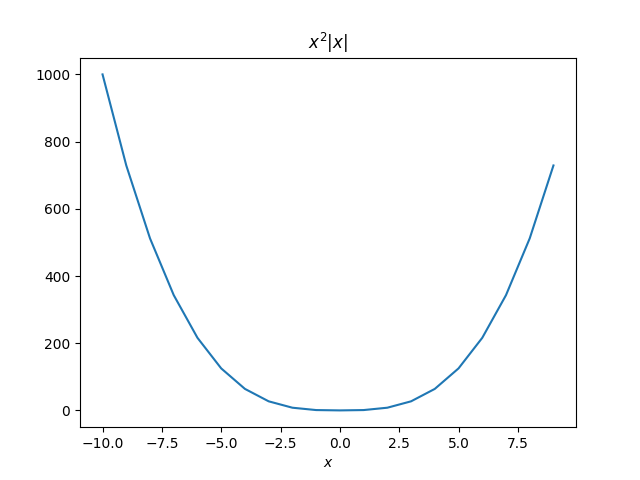
\includegraphics[width=0.4\textwidth]{courbe.png}
        \end{center}
            \caption{$x^2.|x|$}
            \label{courbe}
    \end{figure}

    \paragraph{Stricte convexité du critère du problème \ref{pb:19} :} Pour les mêmes arguments, puis-ce que $q_c \mapsto q^{(0)} + Bq_c$ est une fonction convexe et par composition d'une fonction linéaire et d'une fonction convexe : le critère du problème \ref{pb:19} est convexe.

    \paragraph{Unicité de la solution du problème \ref{pb:19} :} Le critère est strictement convexe, s.c.i, cooercif puis-ce que $<p_r, q^{(0)} + Bq_c> = 0(<q^{(0)} + Bq_c, r\circ q^{(0)} + Bq_c \circ|q^{(0)} + Bq_c|>)$ et donc admet une unique solution, d'après le théorème \textbf{5.3} du cours.\\
    On en déduit alors, par équivalence des problèmes \ref{pb:14} et \ref{pb:19} que le problème \ref{pb:14} admet au moins une solution qui est unique par la stricte convexité du critère.


\section{Séances 2 et 3 - Implémentations d'algorithmes}

    Nous avons cherché à résoudre le problème d'optimisation avec différents algorithmes vus en cours :
    \begin{itemize}
        \item Mise en place d'une recherche linéaire vérifiant les conditions de Wolfe avec l'algorithme de Fletcher-Lemaréchal. Cette étape permet de trouver un pas optimal et conduit notamment à l'\textbf{algorithme de gradient à pas variable}.
        \item Mise en place de l'algorithme de \textbf{Polak-Ribière}, algorithme de gradient conjugué non-linéaire où la direction étudiée dépend de la direction de l'étape précédente.
        \item Mise en place de \textbf{l'algorithme de BFGS} (Broyden-Fletcher-Goldfarb-Shanno) qui est une méthode de quasi-Newton où on utilise une approximation de l'inverse du Hessien de la fonction à minimiser.
        \item Mise en place de \textbf{l'algorithme de Newton} qui n'approxime pas l'inverse du Hessien
    \end{itemize}

    \paragraph{}Nous avons obtenu les résultats présentés sur la Figure \ref{fig:courbes} et synthétisés sur le Tableau \ref{comparAlgo}. Nous remarquons notamment les points suivants :
    \begin{itemize}
        \item L'ajout de la recherche linéaire via l'algorithme de Fletcher-Lemaréchal est une très bonne amélioration qui demande un peu plus de calculs par itération mais en en faisant près de $10\times$ moins demeure deux fois plus rapide qu'un algorithme de gradient à pas fixe.
        \item L'algorithme de Newton est extrêmement rapide (6 itérations) mais demande une bonne connaissance du problème (le Hessien) : toutefois une approximation de ce Hessien, comme à travers l'algorithme BFGS donne également d'excellents résultats.
        \item L'initialisation dans l'algorithme de Fletcher-Lemaréchal est importante. Si on initialise avec le $\alpha$ précédent, comme sur la Figure \ref{fig:pas_variableAlpha}, alors la convergence est très mauvaise.
        \item On remarque que l'algorithme de Fletcher-Lemaréchal fait osciller le pas de gradient.
    \end{itemize}

    
    \begin{figure}
        \begin{subfigure}[t]{0.4\textwidth}
            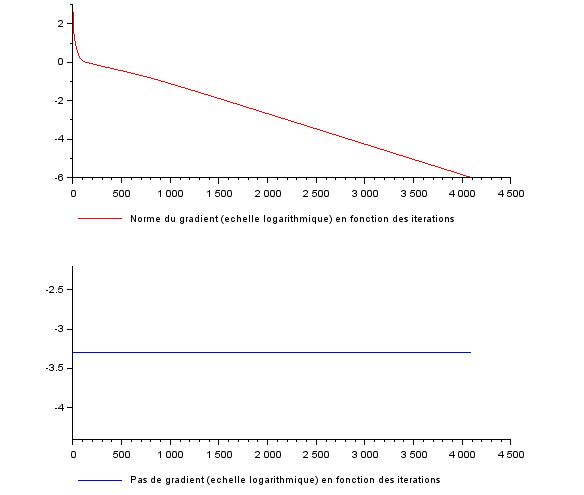
\includegraphics[width=\textwidth]{../Images/Pas_fixe.png}
            \caption{Gradient à pas fixe}
            \label{fig:pas_fixe}
        \end{subfigure}
        \hfill
        \begin{subfigure}[t]{.4\textwidth}
            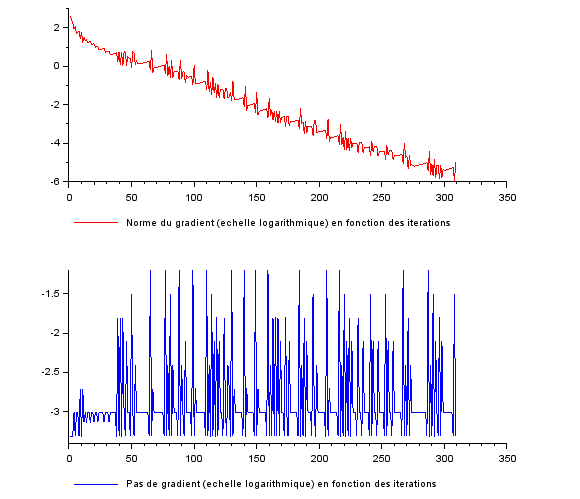
\includegraphics[width=\textwidth]{../Images/Pas_variable.png}
            \caption{Gradient à pas variable (conditions de Wolfe)}
            \label{fig:pas_variable}
        \end{subfigure}
        \hfill
        \begin{subfigure}[t]{.4\textwidth}
            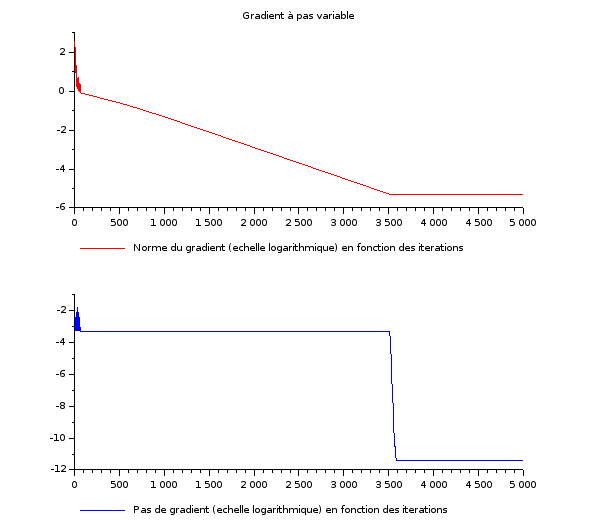
\includegraphics[width=\textwidth]{../Images/pas_variable_initAlpha.png}
            \caption{Gradient à pas variable où Fletcher-Lemaréchal initialité avec $\alpha$ précédent}
            \label{fig:pas_variableAlpha}
        \end{subfigure}
        \hfill
        \begin{subfigure}[t]{.4\textwidth}
            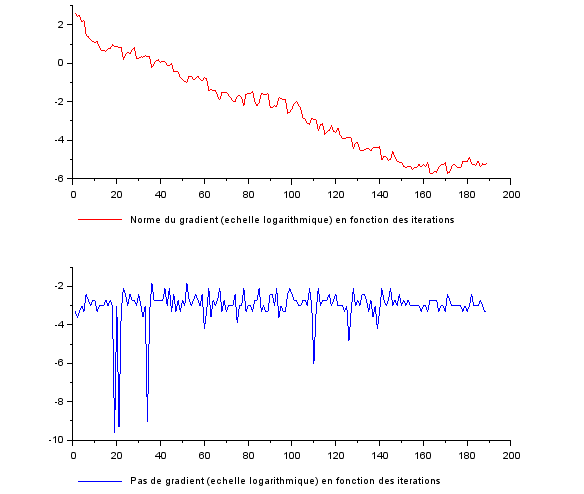
\includegraphics[width=\textwidth]{../Images/Polak_Ribiere.png}
            \caption{Polak-Ribière}
            \label{fig:Polak_Ribiere}
        \end{subfigure}
        \hfill
        \begin{subfigure}[t]{.4\textwidth}
            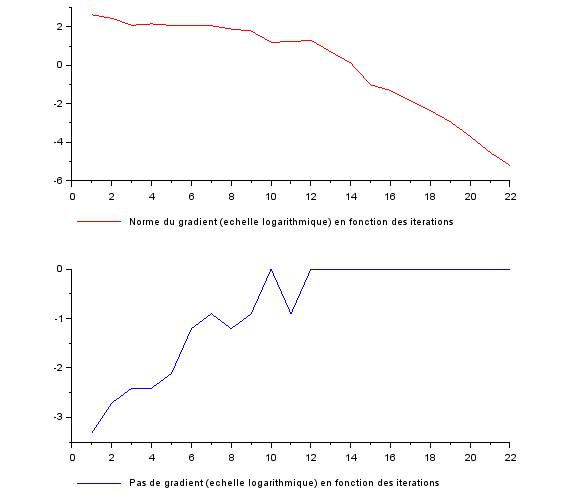
\includegraphics[width=\textwidth]{../Images/BFGS.png}
            \caption{BFGS}
            \label{fig:BFGS}
        \end{subfigure}
        \hfill
        \begin{subfigure}[t]{.4\textwidth}
            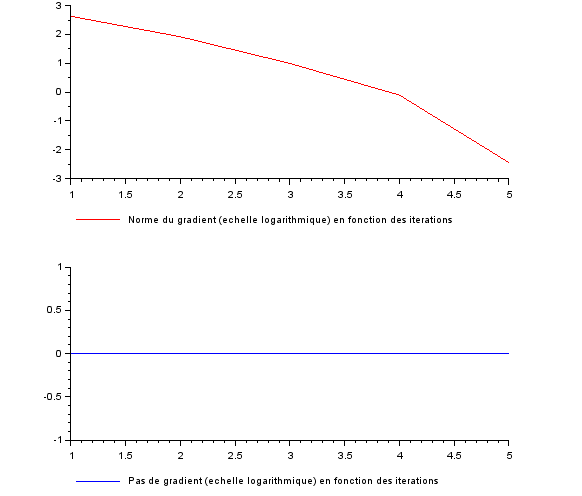
\includegraphics[width=\textwidth]{../Images/Newton.png}
            \caption{Newton}
            \label{fig:BFGS}
        \end{subfigure}
        \caption{Comparaison des différents algorithmes implémentés}
        \label{fig:courbes}
    \end{figure}
    \begin{figure}

        \begin{tabular}{|c|cccccc|}
            \hline
            Méthode & Scilab & Pas fixe & Pas variable & Polak-Ribiere & BFGS & Newton \\
            \hline 
            Itérations & - & 4094 & 310 & 190 & 23 & 6\\
            Temps CPU (s) & 0 & 0.34375 & 0.15625 & 0.109375 & 0.03125 & 0\\
            Critère optimal & -3.734007 & -3.734007 & -3.734007 & -3.734007 & -3.734007 & -3.734007\\
            Norme du gradient & $10^-7$ & $10^-6$ & $9.10^-7$ & $7.10^-7$ & $4.10^-7$ & $7.85.10^-8$\\
            \hline
        \end{tabular}
        \caption{Comparaison des différents algorithmes}
        \label{comparAlgo}
    \end{figure}

    \section{Séance 4 - Minimisation du problème contraint}
        \paragraph{Q.1} Le lagrangien du problème \textbf{14} s'écrit : 
        \[ \mathcal{L}(\lambda, q) = \frac{1}{3}<q, r \circ q \circ |q|> + <p_r, A_rq>
                                    + <\lambda, A_dq - f_d> \]
        
        Les conditions nécessaires d'optimalité sont, étant donné que $\mathcal{L}$ est différentiable :
        \[ \nabla \mathcal{L}_q  = 0
            \text{ et } 
            \nabla_\lambda \min_q \mathcal{L}(q, \lambda) = 0 \]
        
        La première condition se réécrit : 
        \[ 0 = \nabla \mathcal{L}_q  = r \circ q \circ |q| + A_r^Tp_r + A_d^T\lambda \]

        Ce qui se réécrit, correspondant à \textbf{l'expression 8} :
        \[ 0 = r \circ q \circ |q| + A^Tp \]

        où l'on note :
        \[ A = (A_r, A_d)^T \text{ et } p = (p_r, \lambda)^T \]

        La deuxième condition d'optimalité s'écrit, où $\hat{q}$ est un minimiseur de $\mathcal{L}$ :
        \[ A_d \hat{q}(\lambda) - f_d = 0 \]

        Puis, comme $f_r = A_r \hat{q}$, on retrouve \textbf{l'expression 6} :
        \[ A \hat{q} = f \]

        \paragraph{Q.2.} D'après l'expression vérifiée par $\hat{q}$, on peut l'obtenir de manière explicite.
        On introduit pour cela le vecteur $\epsilon$ des signes :
        \[\epsilon_i = -\frac{1}{r_i}(A^T.p)_i\]

        Et on obtient : 
        \[ \boxed{q_i = \epsilon_i \sqrt\left| \frac{1}{r_i}\left(A^T.p\right)_i\right|}\]

        La fonction duale $\Phi(\hat{q}) = \min_q \mathcal{L}(q, \lambda)$ s'écrit alors :
        \[\boxed{\Phi = \frac{1}{3}<\hat{q}(\lambda), r \circ \hat{q}(\lambda) \circ |\hat{q}(\lambda)|> + <p_r, A_r\hat{q}(\lambda)>
        + <\lambda, A_d\hat{q}(\lambda) - f_d>}\]
        
        Le Hessien se calcule comme suit :
        $$ \Phi (\lambda) = \mathcal{L} (q^{\#}, \lambda) $$
        $$ \nabla_{\lambda} \Phi (\lambda) = A_d q^{\#} - f_d $$

        $$ H_{\lambda} \Phi (\lambda) = \nabla_q (A_d q^{\#} - f_d) \nabla_{\lambda} q^{\#} $$

        Or, on peut exprimer la jacobienne de $q^{\#}$ par rapport à $\lambda$ en remarquant que :

        $$ \frac{\partial}{\partial \lambda_j} (r_i\circ q_i^{\#}\circ |q_i^{\#}|) = - (A_d^T)_{ij} $$
        
        $$ \frac{\partial q_i^{\#}}{\partial \lambda_j} = \frac{-1}{2r_i\circ |q_i^{\#}|} (A_d^T)_{ij} $$

        $$ \nabla_{\lambda} q^{\#} = \frac{-1}{2} diag\big(\frac{1}{r_i\circ |q_i^{\#}|}\big) A_d^T $$


        Et alors on obtient :
        $$\boxed{H_{\lambda} \Phi (\lambda) = \frac{-1}{2} A_d diag\big(\frac{1}{r_i\circ|q_i^{\#}|}\big) A_d^T} $$

        \paragraph{Q4.} On observe sur la figure \ref{fig:courbes_dual} les résultats suivants, synthétisés sur le tableau \ref{comparAlgodual}
        \begin{itemize}
            \item Le nombre d'itérations pour résoudre le problème est bien plus important pour le problème dual que pour le problème primal. Par exemple, lorsque le primal avec le méthode à pas-variable met 310 itérations pour converger, le primal ne converge pas en 5000 itérations : il y a presque un facteur 10 entre la résolution du primal et celle du dual.
            \item Les temps CPU sont plus importants pour la résolution du problème dual que pour le problème et cela n'est pas uniquement dû au nombre d'itérations
            \item Pour la méthode à pas-fixe, il faut recalibrer le pas pour avoir une convergence relativement correcte : on a choisi 0.6.
            \item Les allures générales des courbes ne sont pas les mêmes pour la résolution du primal et celle du dual.
            \item La résolution du problème primal de \ref{pb:19} et du dual de \ref{pb:14} conduisent bien au même résultat (au signe - près, puis-ce que nous avons préféré résoudre un problème de maximisation plutôt que de minimisation).
        \end{itemize}

        \begin{figure}
            \begin{subfigure}[t]{0.4\textwidth}
                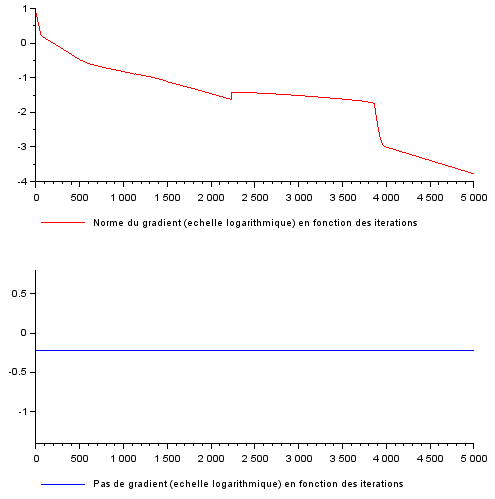
\includegraphics[width=\textwidth]{../Images/Pas_fixe_dual.png}
                \caption{Gradient à pas fixe (pas $\alpha = 0.6$)}
                \label{fig:pas_fixe_dual}
            \end{subfigure}
            \hfill
            \begin{subfigure}[t]{.4\textwidth}
                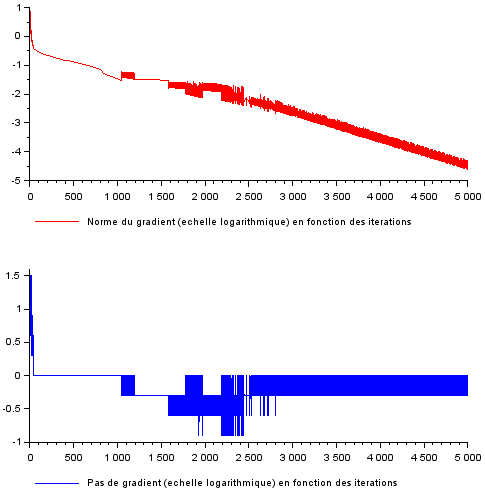
\includegraphics[width=\textwidth]{../Images/Pas_variable_dual.png}
                \caption{Gradient à pas variable (conditions de Wolfe)}
                \label{fig:pas_variable_dual}
            \end{subfigure}
            \hfill
            \begin{subfigure}[t]{.4\textwidth}
                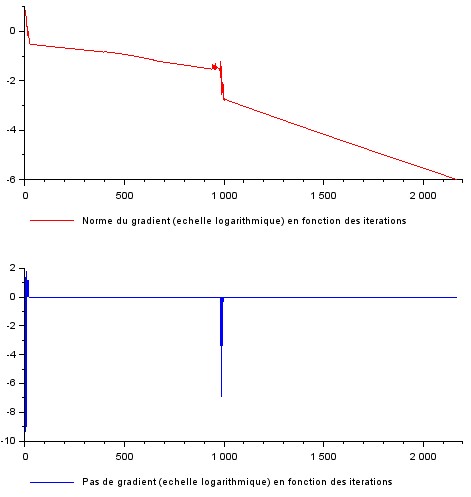
\includegraphics[width=\textwidth]{../Images/Polak_Ribiere_dual.png}
                \caption{Polak-Ribière}
                \label{fig:Polak_Ribiere}
            \end{subfigure}
            \hfill
            \begin{subfigure}[t]{.4\textwidth}
                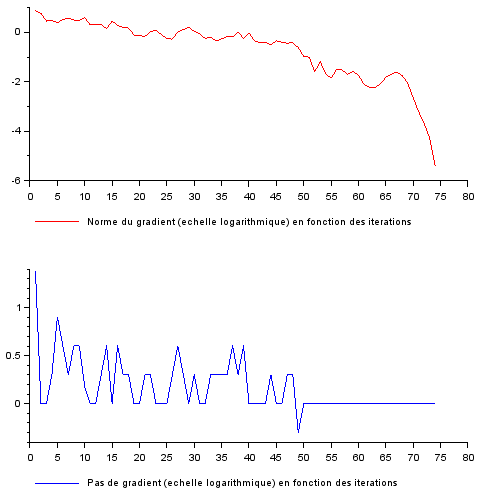
\includegraphics[width=\textwidth]{../Images/BFGS_dual.png}
                \caption{BFGS}
                \label{fig:BFGS_dual}
            \end{subfigure}
            \hfill
            \begin{subfigure}[t]{.4\textwidth}
                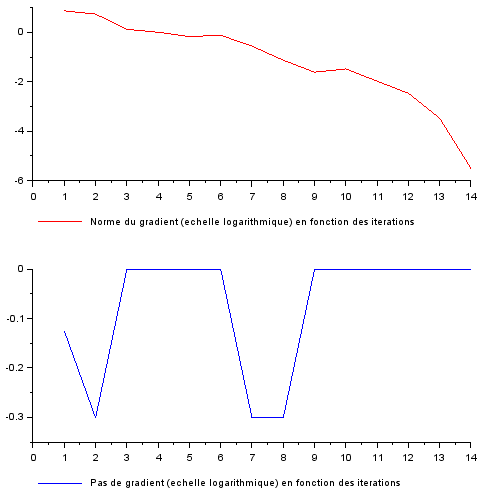
\includegraphics[width=\textwidth]{../Images/Newton_dual.png}
                \caption{Newton}
                \label{fig:Newton_dual}
            \end{subfigure}
            \caption{Comparaison des différents algorithmes implémentés sur le problème dual}
            \label{fig:courbes_dual}
        \end{figure}

     
        \begin{figure}
            \begin{tabular}{|c|cccccc|}
                \hline
                Méthode & Scilab & Pas fixe & Pas variable & Polak-Ribiere & BFGS & Newton \\
                \hline
                Itérations & - & 5000 & 5000 & 2092 & 78 & 17\\
                Temps CPU (s) & 0 & 0.4375 & 0.92187 & 0.46875 & 0.04687 & 0\\
                Critère optimal & - & 3.73401 & 3.734007 & 3.734007 & 3.734007 & 3.734007\\
                Norme du gradient & $10^-7$ & $10^-4$ & $9.10^-7$ & $7.10^-7$ & $4.10^-7$ & $7.85.10^-8$\\
                \hline
                \end{tabular}
            \caption{Comparaison des différents algorithmes pour l'algorithme dual}
            \label{comparAlgodual}
        \end{figure}
    
\end{document}

